\documentclass[twocolumn, traditabstract]{aa}  

\usepackage{fixltx2e}
\usepackage[english]{babel}
\usepackage{graphicx,amsmath}
\usepackage{epstopdf}
\usepackage{epsf,color}
\usepackage[mathscr]{eucal}
\usepackage{amsmath}
\usepackage{amssymb,amsfonts}
\usepackage{natbib}
\usepackage{txfonts}
\usepackage{dsfont}
\definecolor{Mygreen}{rgb}{0.00, 0.72, 0.0}
\definecolor{Mypink}{rgb}{1.0, 0.0, 0.5}
\usepackage[breaklinks, citecolor=blue, linkcolor=Mygreen, urlcolor=Mypink, colorlinks=true, debug, baseurl=' ']{hyperref}
\usepackage{float}
\usepackage{color}
\usepackage{scrextend}
\usepackage{nccmath}
\usepackage{mathtools, cuted}
\usepackage{lscape}
%\usepackage{widetext}
\usepackage{flushend}
\usepackage[T1]{fontenc}
\usepackage{gensymb}
\usepackage{diagbox}



\newcommand{\nika}{{\it NIKA}}
\newcommand{\nikad}{{\it NIKA2}}
\newcommand{\Q}{\mathcal{Q}}
\newcommand{\I}{\mathcal{I}}
\newcommand{\U}{$U$}
\newcommand{\di}{d\mathcal{I}}
\newcommand{\dq}{d\mathcal{Q}}
\newcommand{\eps}{$\varepsilon$}
\newcommand{\epsCMB}{$\varepsilon_{CMB}$}
\newcommand{\epsDET}{$\varepsilon_{det}$}
\newcommand{\rf}{$Rfd\mathcal{I}d\mathcal{Q}$}
\newcommand{\cf}{{\it Cf}}
\newcommand{\todo}[1]{\textcolor{red}{\textbf{#1}}}
\newcommand{\planck}{{\it P\small{LANCK}}}
\newcommand{\healpix}{{\it HEALPix}}
\newcommand{\spice}{{\it SPICE}}

\def\simlt{\lower.5ex\hbox{$\; \buildrel < \over \sim \;$}}
\def\simgt{\lower.5ex\hbox{$\; \buildrel > \over \sim \;$}}
\def\NIKA{\textit{NIKA}}

\bibpunct{(}{)}{;}{a}{}{,}
\bibliographystyle{aa}

\begin{document}
\title{KID systematics and CMB polarization blabla}
\author{A.~Andrianasolo \inst{\ref{IPAG}}\thanks{Corresponding author:
  Aina Andrianasolo, \url{aina.andrianasolo@univ-grenoble-alpes.fr}}
\and  N.~Ponthieu \inst{\ref{IPAG}}
\and  F.-X.~D\'esert \inst{\ref{IPAG}}
\and  M.~Calvo \inst{\ref{Neel}}}

\institute{
Univ. Grenoble Alpes, CNRS, IPAG, F-38000 Grenoble, France 
  \label{IPAG}
    \and
Institut N\'eel, CNRS and Universit\'e Grenoble Alpes, France
  \label{Neel}
}


\date{Received \today \ / Accepted --}
	
\abstract{Here goes the abstract}
\titlerunning{KIDs systematics}
\authorrunning{TBD}
\keywords{Techniques: polarization -- KIDs --  individual: NIKA }
\tableofcontents
\maketitle


\section{Introduction}
\label{sec:introduction}

%Pour citer les papiers: \citep{planck2013mission} ou alors
%\citep{2010A&A...518L.100M,arzoumianian}.


%\begin{itemize}
%\item Why we want to measure CMB polarization B modes
%\item The need for matrices and the KID solution, quickly mention other
%  solutions and multiplexing
%\item Importance to master systematic effects (ref. to previous papers)
%\item KIDs are a new technology that has not yet reached a ``space proof''
%  maturity. In this paper, we address a few specific systematics to KIDs.
%\item Outline
%\end{itemize}


Precise measurement of the cosmic microwave background (CMB) predicted by the $\Lambda$CDM model is one of the major challenges in cosmology. In fact, the CMB anisotropies represent an essential source of information on the physics of the early Universe as it will help us determine the origin of large scales structure and constrain the cosmological parameters of the $\Lambda$CDM model. Since the discovery of the CMB (PENZIAS), several experiments, COBE \citep{1992ApJ...396L...1S}, WMAP \citep{2013ApJS..208...20B}, Planck \citep{2016A&A...594A...1P}, have made precise measurement of CMB temperature anisotropies. These detections have permitted to support the predictions of the $\Lambda$CDM model concerning the primordial nucleosynthesis, formation of structure and on inflation, however these measurements alone can not determine all of the cosmological parameters. The next objectif for the CMB community is the measurement of the CMB polarization and in particular the detection of $B$ modes polarization. The key motivation for CMB polarization measurements is that  inflation models predict the generation of a gravitational wave background. It has been shown that a primordial gravitational wave background would leave an imprint on the polarization pattern of the CMB in the form of B mode polarization \citep{1997PhRvD..55.1830Z, 1997PhRvD..55.7368K}. The measurement of B mode polarization induced by primordial gravitational wave would then provide a powerful probe of inflation. The level of B modes is characterized by the tensor-to-scalar ratio, $r$. The current upper limit on $r$ is < 0.07 ($95 \%$ confidence) \citep{2016PhRvL.116c1302B}. Several missions focused on the detection of B modes, such as LiteBIRD \citep{2014JLTP..176..733M} or COrE \citep{2011arXiv1102.2181T}, are proposed with the objectif of having a sensitivity to be able to detect B modes at the level of $r \sim 10^{-3}$. The level of B mode polarization is several order of magnitude below the level of temperature fluctuations and unpolarized foregrounds, consequently, B modes can easily be degraded by various systematic effect due for exemple to temperature to polarization leakage. Together with high sensitivity, an instrument aiming at measuring the B modes requires a strict control of systematic effects.  
Some of these effects can be reduced in the design of the instruments while others have to be simulated and corrected a posteriori. Numerous systematic effects arise from optical and instrumental imperfections, temperature drifts of the optics and detectors, coupling between instrument imperfections and astrophysical foregrounds and the detector non-linearity. These effects can be modelled and characterized by the spurious signal $C_{l}$ they produce \citep{2008PhRvD..77h3003S,quickpol}. \\
The faintness of B modes signal requires the need to study the Universe at high sensitivity. To do so, the development of large detector arrays is required. Most of the detectors currently used are bolometers such as Transition Edge Sensors (TES), they are installed on experiments such as POLARBEAR \citep{2014ApJ...794..171P} or EPIC \citep{2008arXiv0805.4207B}. Performances of current bolometers are reaching the CMB photon noise limit. The need to build large detector arrays necessitate the development of detectors adapted to strong frequency domain multiplexing. In this context, TES are limited and a new kind of detectors was developed : the Kinetic Inductance Detectors (KIDs), proposed by \citet{2003Natur.425..817D}. Since 2007, these detectors have been developed for the construction of NIKA2 and its prototype NIKA (New IRAM Kids Arrays), which is the first operational instrument using KIDs \citep{2010A&A...521A..29M,2016JLTP..184..816C}. The main characteristic that makes KIDs one of the best candidates to large size detector array is their natural multiplexing capability. Indeed, the resonant frequencies of a resonator can be easily controlled during the array design, and the sharpness of the resonances allows many resonators to be placed into a limited bandwidth. Thus, a large number of resonators, can be coupled to a single transmission line, each one resonating at a different frequency $f_{0}^{i}$ \citep{2010A&A...521A..29M,Calvo2008}.\\
In this paper, we adress specifically the issue of non-linearity. This issue has so far not been addressed in the literature and is of particular relevance to the way KIDs are read out. Many polarization experiments such as POLARBEAR \citep{2017JCAP...05..008T} and \nika2 \citep{2017A&A...599A..34R} use a half wave plate (HWP) to improve the sensitivity in polarizatioon measurements, however the modulation of the HWP induces a strong parasitic signal that is several order of magnitude higher than the noise level. In this paper we will also adress the question of non-linearity that can be brought by this parasitic signal. These issues complement the list of specifications that must be put in instrumental designs in view of a space mission.\\
The paper is organized as follows:
Sect. \ref{sec2} presents a brief description of KIDs...

\section{Measurement of the CMB...}

\subsection{Introduction of the problem and main equations}
\begin{itemize}
\item equations pour montrer l'impact de la non linearite
\item plot qui montre le niveau de NL tolerable sur du CMB pur (les Cl actuels)
  et le niveau de residus de foregrounds qu'on peut tolerer aussi (TE, EB,
  TB...)
\item Do not forget the dipole (NL on it and induced NL)
\item Careful with the actual (single sky) correlation between foregrounds and
  CMB that does not cancel ou ``on stat average''...
\item discuss the maximum expected flux from the galaxy vs a few planet fluxes
  for which we may encounter stronger than spec non linearities.
\item careful not to fit the circle and a small signal (=> bad fit and false
  NL), but to fit it on ``decent signal'' (not too strong either) and THEN
  measure a weak signal. White noise should be enough ?
\end{itemize}

\subsection{Simulations}
\subsubsection{CMB NL residuals}

\subsubsection{Foregrounds residuals}

\begin{itemize}
\item compute foregrounds' alms (polarized) and propagate to power spectra =>
  take 353GHz dust polarized map and 30GHz (which is best) synchrotron
  template. Warning: ringing vs large scale domination
\end{itemize}


\section{Kinetic Inductance Detectors}
\label{se:kids}


%\subsection{Presentation rapide des detecteurs}
%\subsection{Photometrie}
%\subsubsection{Rf}
%\subsubsection{Cf}
%
%\subsection{Non linearite par l'observation d'une source ponctuelle}

%%%%



Kinetic Inductance Detectors (KID) are a novel superconducting detector technology
that provides high sensitivity and ease of multiplexing. In this section we give
a brief summary of their main features and how photometry can be derived from
their measurements.

\subsection{Transfer function}

KIDs are RLC superconducting resonators made from a thin metal film. When
photons are absorbed by the superconducting film, they break Cooper pairs which
increases the quasi-particles density and causes a change in the kinetic
inductance $L_{k}$. This produces a shift $\delta f_{0}$ of the resonant
frequency of the KID \citep{2013A&A...551L..12C} that can be related to the
absorbed optical power $\delta P_{opt}$ (cf.~Fig.~\ref{fig:resonance}). This
relation is linear for small variations in $P_{opt}$
\citep{2010ApPhL..96z3511S}. The KID transfer function is given by:

\begin{equation}
S_{21}(f) = \mathcal{I} +j\mathcal{Q} .
\end{equation}

\noindent where $\mathcal{I}$ and $\mathcal{Q}$ give respectively the real (in phase) and imaginary
(quadrature) of $S_{21}$. A model of a KID transfer function has been proposed
by \citet{2008ApPhL..93m4102G} :

\begin{equation}
S_{21} = \frac{2Z_{res}Z_{0}}{Z_{res}[2Z_{0} + j(X_{1}+X_{2})] + (Z_{0} +jX_{1})(Z_{0} +jX_{2})},
\end{equation}

with:

\begin{equation}
Z_{res} = \frac{Z_{0}Q_{e}}{2Q_{i}}[1 + 2jQ_{i}\frac{(f-f_{0})}{f_{0}}],
\end{equation}

\noindent where $X_{1}$, $X_{2}$, $Z_{0}$ are impedances, $Q_{i}$ is the
intrinsic quality factor of the resonator and $Q_{e}$ is the external quality
factor due to coupling with the measurement electronics. $f$ is the frequency of
excitation of the detector, and $f_{0}$ is the resonant frequency. Throughout
this paper, we shall assume typical values of KIDs $X_{1} = X_{2} =
0.5\,\Omega$, $Z_{0} = 50\,\Omega$, $Q_i=2\times 10^4$, $Q_e=10^4$ and $f_{0} =
1.8\times 10^9$\,Hz as measured on \nika\ and \nikad. The following section
addresses how the resonance of a KID is monitored and related to the incident
optical power.

\begin{figure}
  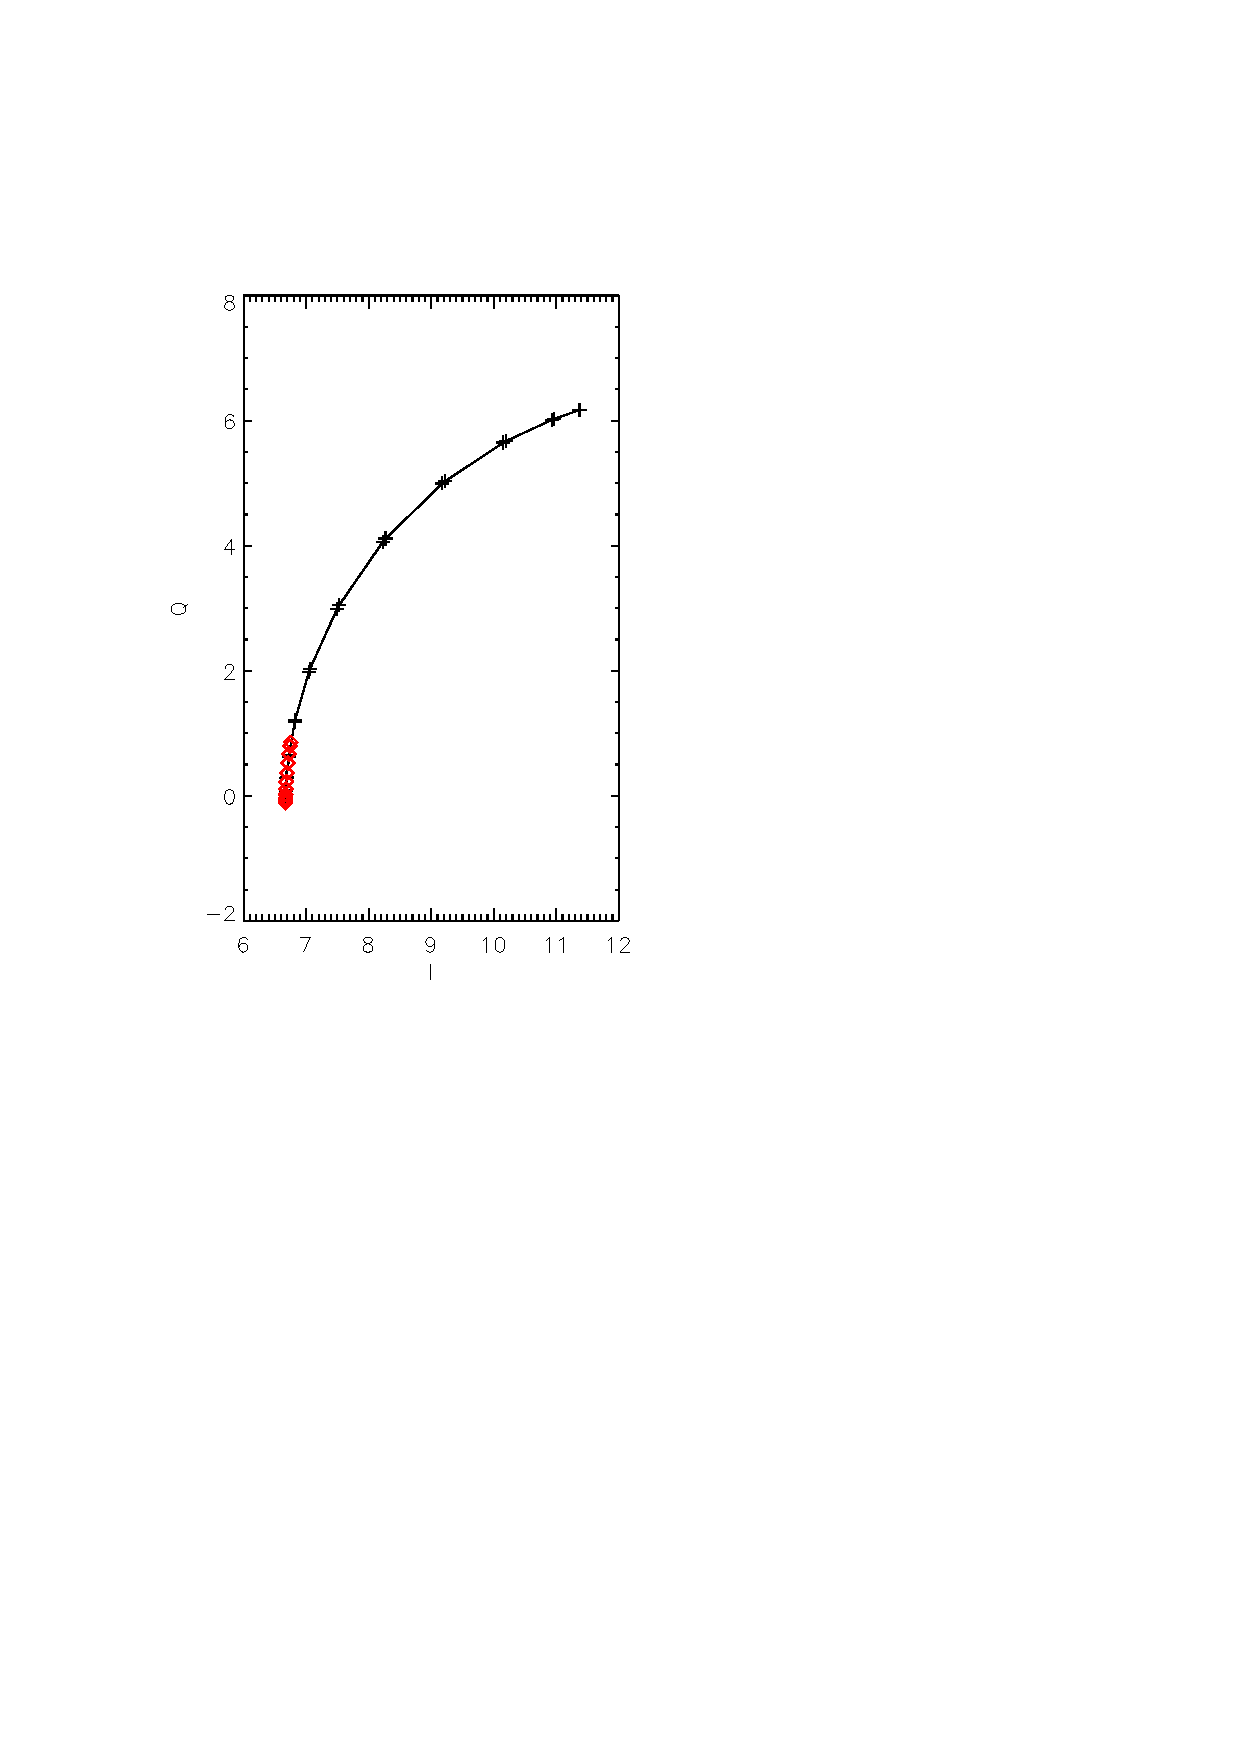
\includegraphics[clip, angle=0, width=\columnwidth]{Figures/resonance.png}
  %	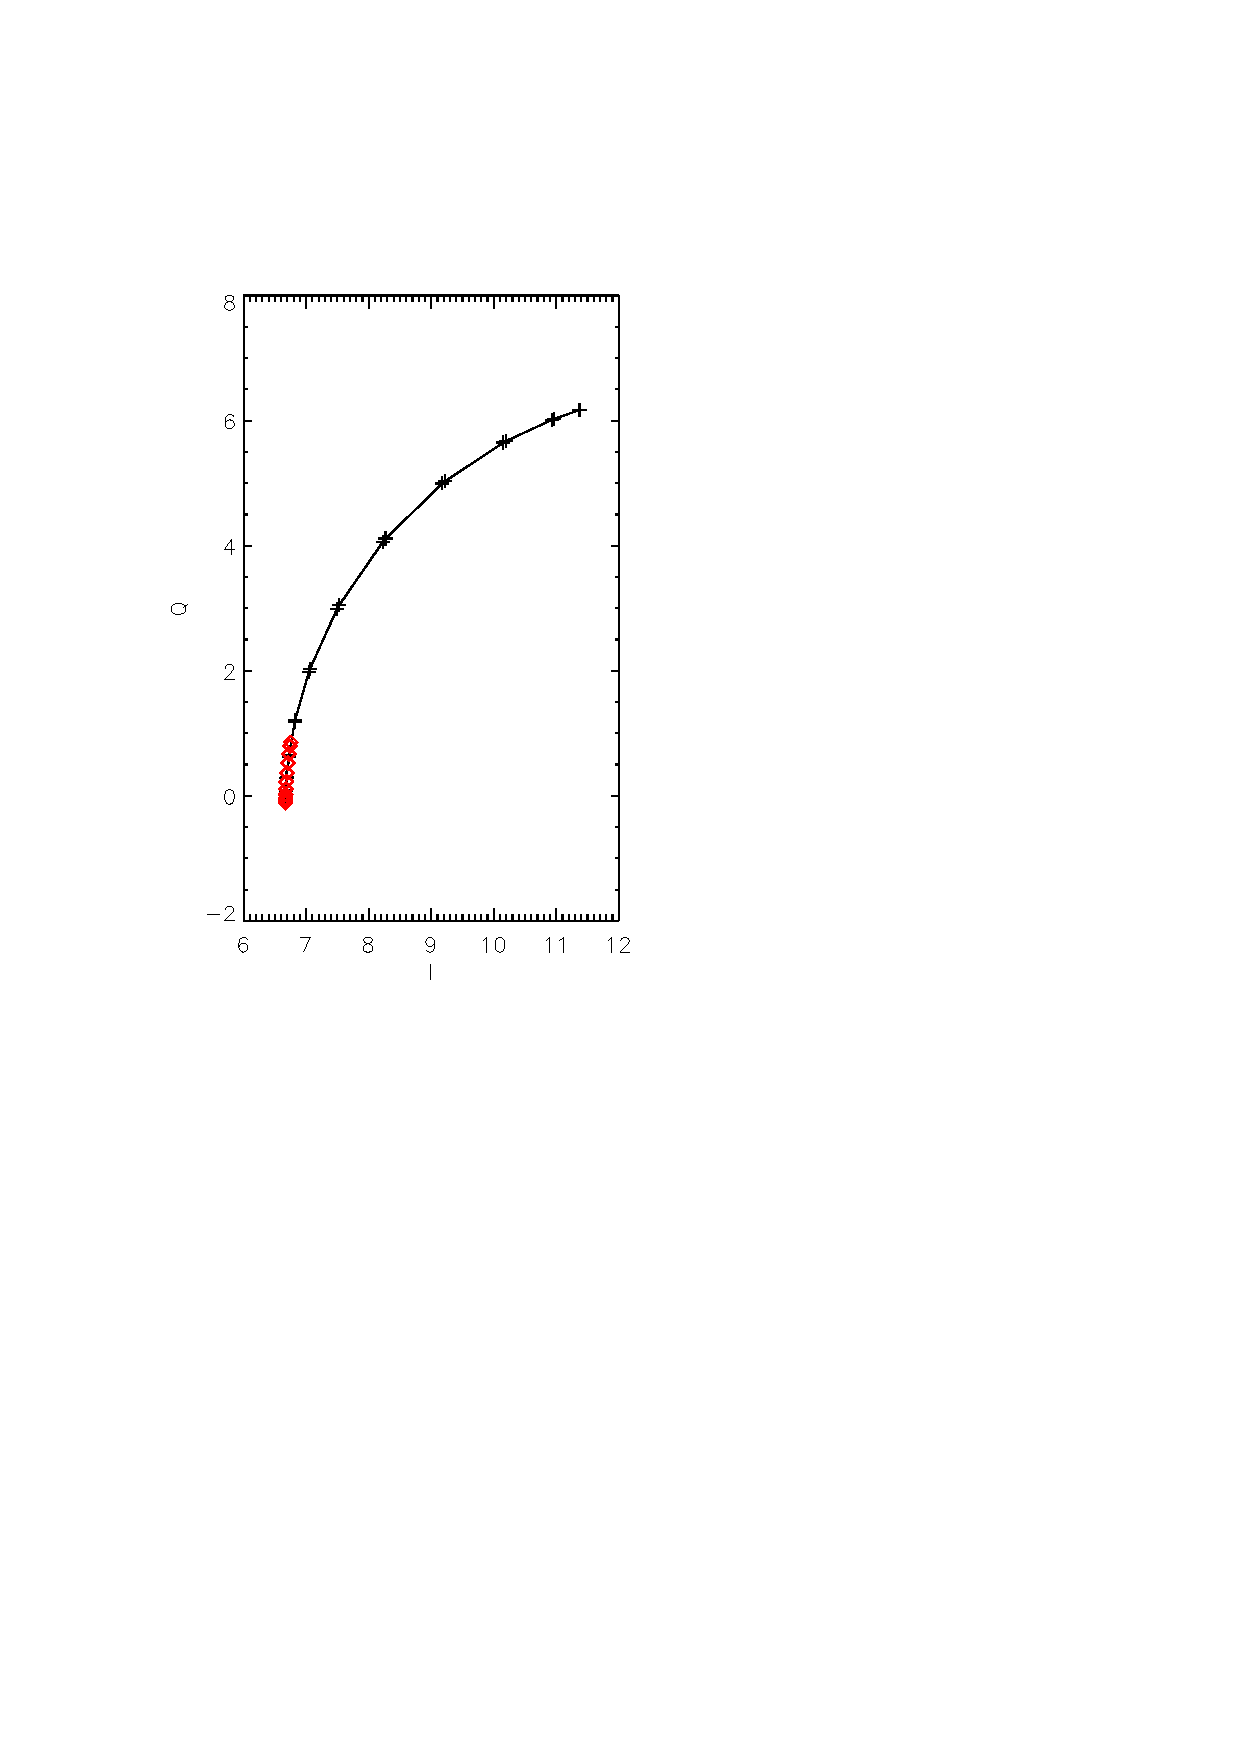
\includegraphics[clip, angle=0, width=\columnwidth]{Figures/resonance.pdf}
  \caption{Schematic representation of a KID resonance in amplitude (left) and phase (right), as a function of the excited tone injected in the feedline. The optical power absorbed by the detector is weak for black curves and increases for red curves. The absorption of a photon shifts the resonance frequency and this is directly proportional to the received power.}
  \label{fig:resonance}
\end{figure}



% \section{Methods of signal reconstruction}
\subsection{Photometry}
\label{sec:signal}

A dedicated KID readout system has been developed by \citet{2013A&A...551L..12C}
and successfully used for \nika\ and \nika2\ \citep{2010A&A...521A..29M,2016JLTP..184..816C}. We here summarize its main charcteristics and the observables
that are relevant for our simulation work. We then present two ways to use them
to derive the photometry.

%% To convert the $\I(t)$ and $\Q(t)$ that
%% describe the resonance frequency shift $\delta f_0$ to the absorbed optical
%% power $\delta P_{opt}$. We have devised two ways to relate these
%% quantities. Both rely on a specific electronic modulation readout devised by
%% \citet{2013A&A...551L..12C} that we summarize first.

\subsubsection{Modulated readout technique}

\begin{figure}
  \includegraphics[clip,angle=0,width=\columnwidth]{Figures/resonance-circle.png}
  \caption{Trajectory of $\I$ and $\Q$ during a frequency sweep around the
    resonance of a KID. The arrows represent $(\di,
    \dq)$. \citep{2013A&A...551L..12C}}
  \label{circle-iq}
\end{figure}

The excitation tone frequency of a KID is modulated by a local oscillator with a
known frequency shift. This provides two values $f_{\pm} = f_0 \pm \delta
  f_{LO}/2$ with $\delta f_{LO} \simeq 1$\,kHz. The ``In-phase'' in
``in-Quadrature'' amplitudes $i(t)$ and $q(t)$ then read:

\begin{equation}
(i(t), q(t)) = (\frac{i(f_{+}) +
    i(f_{-})}{2},
\frac{q(f_{+}) + qf_{-})}{2}),
\end{equation}

and the differential values are :

\begin{equation}
\label{gradient}
(\di(t), \dq(t)) =
\left(\frac{i(f_{+}) - i(f_{-})}{\delta f_{LO}},
\frac{q(f_{+}) - q(f_{-})}{\delta f_{LO}}\right).
\end{equation}

These quantities are represented on Fig. \ref{circle-iq}. In this paper, we take
typical laboratory values and assume that $i$ and $q$ are sampled at
880\,Hz. This high acquisition rate is allowed by the sub-millisecond time
constant of the KIDs. For most experiments, such a high sampling rate is not
required and we average these measures over 40~samples to produce
four secondary quantities at 22\,Hz:

\begin{eqnarray}
\I  &=& \sum^{N_{m}=40}_{p=1} i_{p},\\
\Q  &=& \sum^{N_{m}=40}_{p=1} q_{p},\\
d\I &=& \sum^{N_{m}/2=20}_{p=1} i_{2p} - i_{2p-1},\\
d\Q &=& \sum^{N_{m}/2=20}_{p=1} q_{2p} - q_{2p-1}.
\end{eqnarray}

With these quantities in hand we have several ways to derive the transmitted
signal. They are presented in the following paragraph.

\subsubsection{\rf}
If a variation $\Delta\I(t)$, $\Delta\Q(t)$ is observed between successive ($\I$,
$\Q$) points, it is possible to estimate the shift of the resonant frequency
$\Delta f_{0}$ between these two samples by comparing ($\Delta \I$, $\Delta \Q$)
with the gradient $(\di,\dq)$ induced by the known $\delta
f_{0}$ of the local oscillator. This is done by a scalar projection of ($\Delta\I$,
$\Delta\Q$) on $(\di,\dq)$ that is tangent to the resonance circle. To have a
cleaner estimation of the latter, we take its running average over 50
points that we write $\langle . \rangle_{50}$ \citep{2014A&A...569A...9C}:

\begin{equation}
\label{eq:Rf}
\Delta f_{0} = \delta f_{LO} \frac{\Delta \I\, \langle \di
  \rangle_{50}
+ \Delta \Q\, \langle \dq \rangle_{50}}{\langle \di
  \rangle_{50}^{2}
 + \langle \dq \rangle_{50}^{2}},
\end{equation}

Note that this average is performed only on the tangent vector $(\di,\dq)$ so
that $\Delta f_0$ is sampled like $\I$ and $\Q$ at 22\,Hz. This method has been
successfully used in \todo{XXXX}, but can be affected by some systematic
uncertainty and be a source of non-linearity. Indeed, $(\di,\dq)$ is tangent to
the $(\I,\Q)$ circle for a fixed background optical power, while, in principle,
the incident optical power that induces the observable $(\Delta \I, \Delta \Q)$
should distort the resonance circle to some extent. As a consequence, the
observed $(\I,\Q)$ trajectory is not precisely parallel to the $(\di,\dq)$
direction. Early laboratory and on-site tests have shown that this approximaton
leads to a reconstruction of point source fluxes better than 2\%
\citep{2013A&A...551L..12C}. In this work, we improve this upper limit on
simulations and assess the impact of this error on futures CMB polarization
measurements.

\subsubsection{Circle fit : Cf}

\begin{figure}
\includegraphics[clip, angle=0, width=\columnwidth]{Figures/circle_zres.eps}
\caption{Bottom: location of $\I$ and $\Q$ when a KID observes a point source of
  various fluxes. Top: ratio of the distance between $(\I,\Q)$ and the center of
  the fitted circle over the radius of this circle. All the points on the pure
  imaginary line at $\I=1$ are the result of the transformation of the circle
  into $Z_{res}$ according to eqs.~(\ref{eq:z_res}) and
  (\ref{eq:scale_rotate}).}
\label{fig:circle_zres}
\end{figure}

\todo{ref to the circular nature of (I,Q): \cite{2011ApJS..194...24M}}.\\

To improve \rf, we developed a new technique that fully exploits the circular
nature of the $(\I,\Q)$ trajectory, hereafter called \cf. It is
  based on the transformation property of a circle in the complex plane into a
  straight line. Indeed, let us consider a circle centered on $(0,1/2)$ with a
  radius $1/2$ and compute its inverse:

\begin{eqnarray}
Z_{ref} &\equiv&\frac{1}{2} + \frac{1}{2}e^{i\phi}\,, \\
&=&\cos\frac{\phi}{2}e^{i\phi/2}\,,\\
Z_{res} &\equiv& 1/Z_{ref}\,, \label{eq:z_res} \\
&=&1-i\tan\frac{\phi}{2}\,.
\label{eq:z_res}
\end{eqnarray}

$Z_{res}$ is a straight line and along this line $Z$ varies linearly with
$\phi$ for small values of $\phi$. Experimentally, we are in this regime
when the signal is weak and when $\phi$ is defined w.r.t.~ the $(O,C)$ axis
as defined on Fig.~\ref{fig:circle_zres}. We thus fit the radius $r$ and the
center $(\I_c,\Q_c)$ of our measurement circle $Z=\I+j\Q$. Defining
$\alpha=\arctan\Q_c/\I_c$, we scale, rotate and translate this
circle to the $Z_{res}$ circle according to

\begin{equation}
Z_{ref} = \left(\begin{array}{c}
\I_{ref}\\
\Q_{ref}\end{array}\right) = 
\frac{-1}{2r}\left(\begin{array}{rr}
\cos\alpha & \sin\alpha\\
-\sin\alpha & \cos\alpha\end{array}\right)
\left(\begin{array}{c}
\I-\I_c\\
\Q-\Q_c\end{array}\right) +
\left(\begin{array}{c}
1/2\\
0\end{array}\right)
\label{eq:scale_rotate}
\end{equation}

The result of this transformation is shown on Fig.~\ref{fig:circle_zres}. A
variation of the signal $(\Delta\I,\Delta\Q)$ leads to a variation
$\Delta\phi$ along $Z$ that is proportional to the frequency shift $\Delta f$
that we are after to determine photometry. To derive the calibration between
these two quantities, we once again rely on the $(\di,\dq)$ that is induced by
the known $\delta f_{LO}$. Applying transformation (\ref{eq:scale_rotate}) to
$(\di,\dq)$, we obtain the corresponding variation $dy = Im(dZ_{res})$. The
final derivation of $\Delta f$ corresponding to $(\Delta\I,\Delta\Q)$ requires
the integration of $dy/\delta f_{LO}$. For the sake of simplicity, we fit
$Im(dZ_{res})$ as a polynomial of $dy/\delta f_{LO}$ that is therefore trivial
to integrate.

%% \begin{equation}
%% \tan\frac{\delta\phi}{2} \simeq \frac{\delta\phi}{2} +
%% \frac{(\delta\phi)^3}{15}
%% \end{equation}

\subsection{Non linearity characterization with simulations of observations of a point source}

\begin{figure}
\center
\includegraphics[clip, angle=0, width=\columnwidth]{Figures/KID-linearity-Monfardini2014.png}
\caption{KID linearity demonstrated in laboratory under realistic
  conditions. The plot shows the frequency shift of the resonance as a function
  of the optical background temperature (K). Solid line : linear fit of the
  experimental points. Credits : \citet{2014JLTP..176..787M}.}
\label{fig:KID-lin}
\end{figure}

Laboratory measurements with \todo{XXXX describe set up XXX} have shown that
KIDs are linear over a wide range of backgrounds
(Fig.~\ref{fig:KID-lin}). However, for these measurements, $\Delta f$ was not
reconstructed as described in the previous section, and we want to characterize
our formalism up to $\epsilon$ of the order of $10^{-5}-10^{-6} $ TBC.

To characterize KIDs non linearity, we write the non linear detector response as :

\begin{equation}
m^{Rf,Cf} = m + \varepsilon m^2 +c_{0}.
\label{eq:model_kid_nl}
\end{equation}

$\varepsilon$ represents the non linearity of the KID.


We simulate
the measure of point source by a KID and show how linear this measure remains in
various contexts. Non linearity could appear when the source is very bright
(such as planets of several tens of Jy) and the density of charge carriers is
altered. This leads to $(\I,\Q)$ measures that leave the resonance circle, hence
invalidating the approximations made in the photometric equations of the
previous section. A second possible source of non linearity is the instrument
scanning speed. Indeed, even if the source is moderately bright, if it is
scanned too fast, $(\Delta\I,\Delta\Q)$ could be far from the tangent vector
$(\di,\dq)$ which would alter their linear relation. In this paragraph, we
explore both cases.\\

We simulate the observation of a point source with a flux
that we vary between \todo{1 and 2000\,Jy TBC} (fluxes are unrealistically large on purpose for illustration). We assume that our instrument has
a 11\,arcsec FWHM Gaussian beam like the polarized 1\,mm channel of \nikad. We
also vary the scanning speed of our virtual instrument while keeping a minimum
of 3~samples per FWHM to respect the Nyquist criterion.
As shown in Fig.~\ref{fig:planet_profiles} and Fig.~\ref{fig:flux_out_vs_in}, non linearity appears with the distortion of the input gaussian profile in the case of \rf\ method whereas \cf\ remains linear on the same flux scale.

\begin{figure}
  \includegraphics[clip, angle=0, width=\columnwidth]{Figures/planet_profiles.eps}
  \caption{Comparison of an incoming flux that we vary between 1 and 2000 Jy TBC (in black), with flux reconstructed by \rf\ and \cf. Fluxes are unrealistically large on purpose for illustration. }
  \label{fig:planet_profiles}
\end{figure}


\begin{figure}
  \includegraphics[clip, angle=0, width=\columnwidth]{Figures/flux_out_vs_in.eps}
  \caption{Comparison of an incoming flux that we vary between 1 and 2000 Jy TBC (in black), with flux reconstructed by \rf\ and \cf. Fluxes are unrealistically large on purpose for illustration. }
  \label{fig:flux_out_vs_in}
\end{figure}

For all simulations we computed the non-linearity coefficient $\varepsilon$ from eq.~\ref{eq:model_kid_nl} by doing a fit of the input fluxes as a fonction of output fluxes. Results are shown in Tab.~\ref{tab:eps}. As in the two figures the non-linearity coefficients show \rf\ method is less linear than \cf\ on the same flux scale.

\begin{table}
\center
\begin{tabular}{|c|c|c|}
	\hline
	    & $\frac{3pts}{beam}$ & $\frac{5pts}{beam}$ \\
	\hline
\rf\	&  $-4.58 \times 10^{-5}$ & $-2.33 \times 10^{-5}$ \\
	\hline
\cf\ & $1.09 \times 10^{-7}$   & $8.90 \times 10^{-8}$ \\
	\hline
\end{tabular}
\caption{Non-linearity coefficients $\varepsilon$ from an incoming flux that we vary between 1 and 500 Jy.}
\label{tab:eps}
\end{table}

Simulations of a KID exposed to a point source with a large variation of fluxes have shown that it meets the requirement addressed in Sec.~\ref{sec:cmb}. 
HWP presente bcp d'avantages pour les futurs experiences cmb, dans la prochaine section on regarde la NL induite par la HWP. 


\section{Half Wave Plate modulation}

\begin{itemize}
\item les HWP deviennent a la mode
\item les kids ont des constantes tres petites, donc on peut faire tourner vite
  : avantages...
\item ... mais signal parasite tres fort et donc besoin de le soustraire et de
  voir si il n'induit pas de non linearite sur la mesure du signal
\item simulations du HWPSS (beta): bien expliquer que ce qui compte c'est la
  subtraction of this template not the exact recovery of the input model
\item anticipate a bit on the achieved residual NL on the same planet as in the
  previous section.
\end{itemize}


\section{Scanning strategy}

\begin{itemize}
\item explain how the 4f harmonics separates from the scanning frequencies
\item derive constraints on precession, nutation and scanning speed vs HWP
  speed.
\item Number of samples per beam vs combination of kids to produce a map: one
  map is the average of N independent maps *only* if *each* KID produces a full
  map. Otherwise it's a somehow classic combination of different detectors
\end{itemize}

%Here we scan a map of the Galaxy with the two pointing strategies described earlier. In addition to the Galaxy, there is another signal that we have to take into account which is the CMB dipole. The CMB dipole is a smooth gradient in the CMB temperature accross the sky. It is the result of the motion of the local group of galaxies with respect to the reference framed defined by the CMB. The CMB dipole amplitude is $\Delta T = 3.365 \pm 0.027$ mK and directed toward $(l,b) = (264.4 \degree \pm 0.3 \degree , 48.4 \degree \pm 0.5 \degree)$ in galactic coordinates \citep{2015IJMPD..2430004B}. Like in the precedent simulations we add the template of HWP that we subtract after the signal goes through the KID model.
%
%We have seen previously that to be in a linear regime, constraints had to be put on the scanning strategy, especially on the scanning speed, and on the incoming flux. Here the scanning strategy that we use ensure that we respect the Nyquist criteria, by having a number of points per beam between 3 and 5. Plus, we can see in Fig.~\ref{fig:histo-gal-dip}, that the flux of the Galaxy and Dipole does not go higher than 20 Jy and that the two methods \rf\ and \cf\ can reconstruct it.
%
%%% In the context of a CMB experiment mapping a large fraction of the sky, one
%% should also consider the CMB dipole with its 6.73\,mK peak to peak \todo{ADD
%%   REF} converts into a \todo{XXX\,Jy} signal \todo{Account for the bandpass
%%   !!}. It can displace the zero level $Z$ along the circle so that a
%% bright source would enter the non linear regime sooner than expected. This is
%% also true for strong Galactic emission like that of Dust at frequencies above
%% $\sim 100$\,GHz. It is even truer for the background modulation induced by a
%% rotating Half Wave Plate (HWP). After early tests by \todo{cite Hildebrand in
%%   the 80's or so ?}, this kind of modulating device has been left aside for
%% \todo{20~TBC} years in the context of millimetric observations. With the
%% improvement of technologies, it progressively came back in the landscape, in
%% particular with pioneering experiments like \emph{Maxipol}
%% \citep{2007ApJ...665...42J} and \emph{EBEX} \citep{2010SPIE.7741E..1CR}. It is
%% now more and more common and is considered as the leading option for future
%% satellite designs such as \emph{LiteBIRD} \todo{add ref.}. \nika\ has used a
%% fast and continously rotating HWP and saw strong parasitic signal synchronous
%% with the HWP rotation harmonics \citep{2017A&A...599A..34R} like \emph{Maxipol}
%% and \emph{EBEX} (cf.~Fig.~\ref{fig:hwp_power_spectrum}). The amplitude of this
%% signal is comparable to bright planets at several tens of Jy and could also bias
%% the average position of the $Z$ measurement and hence the photometry.


%% \todo{keep for global conclusion:} In conclusion, because we can not directly
%% measure the optical power from a KID, new methods were developed to monitor the
%% shift of the resononance frequency of the detector. First with the modulated
%% readout technique we can calculate four quantities : $\I$, $\Q$, $\di$,
%% $\dq$. With these quantities in hand, we can monitor the shift of the resonant
%% frequency and derive the corresponding incident power ny using the two methods
%% that were developed : \rf\ which is already successfully used in \nika\ and
%% \nika2\ (see \citep{2014A&A...569A...9C}) , and \cf\ which is an improvement
%% from \rf . In this paper, we compare these two methods in terms of linearity. To
%% do so, in the next sections we do simulations of observations by a KID and we
%% use \rf\ and \cf\ to reconstruct the signal. We then study the impact of the KID
%% non-linearity on the search for B modes polarization of the CMB.


\clearpage
\newpage

\section{Conclusion}
\label{conclusion}

\todo{Recall that we are in fact interested in the unknown difference between
  the model and the measure, not specifically its linearity that can be
  considered as a first order approximation to any differnce between an a priori
  known calibration curve}\\

\todo{aussi faire remarquer que l'eq.~(\ref{eq:eq-NL}) is linear in $\epsilon$,
  so we have further mitigation by the average of many detectors around their
  known calibration curve.}\\

This paper presents the study of KIDs systematic effects such as the non-linearity and an application to the CMB polarization. 
KIDs are a new kind of detectors based on superconducting technology that provides high sensitivity. They have been developed for the construction of NIKA and NIKA2 since 2007, which is now the first operational instrument using KIDs. One of the key asset of KIDs is their natural multiplexing capability which makes them one of the best candidates for future space mission that needs large size detector array. In this context, in a first part, we studied the response of a KID by using two methods to reconstruct the signal (\rf and \cf) and its systematic effects caracterized by its non-linearity coefficient \eps. For an incoming source consisting of a planet of 500 Jy, the dipole and a HWP, and for different scan speed, we found $\varepsilon_{rf}$ $\simeq 10^{-5}$ and $\varepsilon_{cf}$ $\simeq 10^{-7}$. The non-linearity depends on the way that we reconstruct the signal, and even if \rf can reconstruct the signal very well, \cf is better at it and generates less non-linearities. Another good point is that the modulation of the HWP does not bias the measurement by inducing large non-linearities. We have seen that in order to have less non-linearities, we need to put constraints on the scanning speed, so in a second part, we did more realistic simulations, by scanning a map of the Galaxy and dipole by using satellite pointing strategies. We found, that depending on the incoming sources, $\varepsilon_{rf}$ varies between $10^{-7}$ (Galaxy only) and $10^{-3}$ (Galaxy, dipole, HWP), and $\varepsilon_{cf}$ varies between $10^{-8}$ (Galaxy only) and $10^{-4}$ (Galaxy, dipole, HWP) (POLSAT, VOIR PB PLANCK). The results show that in a space context KIDs are capable of accurately reproducing the signal and that as in the precedent simulations \cf is slightly better than \rf.\\
The measure of CMB $B$ modes polarization is a major goal of observational cosmology, as their detection would sign the presence of primordial gravitational waves and provide a confirmation of inflation. Observations of CMB polarization demand a high control of systematics effect and in light of this, we demonstrated the capabilities of KIDs arrays to detect B modes polarization by comparing systematic effects coming from the detector and the leakage of dust temperature into polarization maps. With HEALPix, we simulated spurious signals from a map of the Galaxy and generated modified $C_{l}$. From $C_{l}^{TE}$, we calculated the coefficient ($\varepsilon'$) related to the leakage of temperature into polarization. For a tensor-to-scalar ratio (T/S) = 0.1, 0.01, 0.001 we respectively found $\varepsilon' \simeq 2.51$x$10^{-2}$, 7.95x$10^{-3}$, 2.51x$10^{-3}$. Because the leakage of temperature into polarization maps is the systematic effect that is most likely to contaminate the detection of $B$ modes , to be able to measure them, the non-linear coefficient $\varepsilon$ related to the detector must be lower than $\varepsilon'$. In all of the precedent simulations, $\varepsilon $ varried between $10^{-3}$ and $10^{-8}$, so $\varepsilon < \varepsilon'$, therefore we can say that the KID is capable of detecting $B$ mode polarization. Finally, because of the KID multiplexing ability and its capability of detecting $B$ mode polarization, we can say that KID technology is developping toward becoming one of the best candidates to space mission and study of the CMB polarization.

 
\bibliography{biblio}

%-----------------------------------------------------
\begin{acknowledgements}
NIKA standard acknowledgements + FOCUS + E.~Hivon.\\
\todo{Acknowledgement of Planck data:} Based on observations obtained with Planck
(http://www.esa.int/Planck), an ESA science mission with instruments and
contributions directly funded by ESA Member States, NASA, and Canada.
\end{acknowledgements}

\end{document}
